% The contents of this file is 
% Copyright (c) 2009-  Charles R. Severance, All Righs Reserved

\chapter{왜 프로그래밍을 배워야 하는가?}

컴퓨터 프로그램을 만드는 행위(프로그래밍)는 매우 창의적이며 향후 뿌린 것 이상으로 얻을 것이 많다. 프로그램을 만드는 이유는 어려운 자료분석의 문제를 해결하려는 것에서부터 다른사람의 문제를 해결해주는 재미를 느끼는 것까지 다양한 이유가 있다. 이 책에서 모든 사람이 어떻게 프로그램을 만드는지를 알고, 프로그램을 만드는지를 알게되면, 새로 습득한 프로그래밍 기술로 원하는 것을 해결할 수 있는 것을 배우게 된다.

우리의 일상은 노트북부터 핸드폰까지 다양한 컴퓨터에 둘러싸여 있다. 이러한 컴퓨터가 개인비서로 우리를 위해서 많은 일을 대신해 준다고 생각한다. 일상생활에서 접하는 컴퓨터 하드웨어는 우리에게 "다음에 무엇을 하면 좋겠습니까?" 라는 질문을 지속적으로 물어보게 만들어 졌다.


 
\beforefig
\centerline{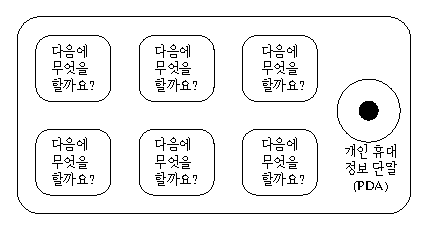
\includegraphics[height=1.00in]{figs2/pda.eps}}
\afterfig

프로그래머는 운영체제와 하드웨어에 응용 프로그램을 만들었고, 결국 많은 것들을 도와주는 PDA(Persoanl Digital Assistant)로 진화했다. 컴퓨터는 빠르며, 큰 저장소를 가지고 있어 우리가 컴퓨터에게 "다음꺼 실행해(do next)를 컴퓨터가 이해할 수 있는 말로 지시를 하게되면 우리에게 매우 유용할 수 있다.

예를 들어, 다음의 세 문단을 보고 가장 많이 나오는 문단의 단어를 찾아보고 얼마나 나오는지를 알려주세요라고 컴퓨터에게 시킬 수 있다. 사람이 몇초만에 단어를 읽고 이해할 수는 있지만, 그 단어가 몇번 나오는지를 세는 것은 매우 고생스렁운 과정이다. 왜냐하면 사람은 지루하고 반복되는 일의 문제를 해결하는데 적합하지 않기 때문이다. 컴퓨터는 정반대이다. 논문이나 책에서 텍스트를 읽고 이해하는 것은 컴퓨터에게 어렵다. 하지만 단어를 세고 가장 많이 사용되는 단어를 말해주는 것은 컴퓨터에게는 무척이나 쉽다.

\beforeverb
\begin{verbatim}
python words.py
Enter file:words.txt
to 16
\end{verbatim}
\afterverb
%
우리의 개인 정보분석 비서는 "to"라는 단어가 가장 많이 사용되었고 16번 나왔다고 바로 답을 준다.

사람이 잘하지 못하는 점을 컴퓨터가 잘할 수 있다는 사실을 이해하면 왜 컴퓨터 언어로 컴퓨터와 대화해야 하는지를 알 수 있다. 컴퓨터와 대화할 수 있는 언어(Python)를 배우게되면 지루하고 반복되는 일을 컴퓨터가 처리하게 하면 더 많은 시간을 창의적이고, 직관적이며, 창조적인 시간을 컴퓨터와 함께 할 수 있다. 

\section{창의성과 동기}
이책은 직업 프로그래머를 위해서 저작된 것은 아니지만, 직업적으로 프로그램을 만드는 작업은 개인적으로나 경제적인면에서 꽤 매력적인 일이다. 특히, 유용하며, 심미적이고, 똑똑한 프로그램을 다른 사람이 사용할 수 있도록 만드는 것은 매우 창의적인 일이다. 컴퓨터는 다양한 그룹의 프로그래머들이 사용자의 관심과 시선을 빼았기 위해서 경쟁적으로 다양한 프로그램을 가지고 있다. 이렇게 개발된 프로그램은 사용자가 원하는 바를 충족시키고 훌륭한 사용자 경험을 주려고 노력한다. 이러한 상황에서 사용자가 소프트웨어를 고르게 될 때 고객의 선택에 대해서 프로그래머는 직접적으로 보상을 받게된다.

만약 프로그램을 프로그래머 집단의 창의적인 결과물로 바라본다면, 아마도 다음의 그림이 PDA 컴퓨터에 의미가 있을 듯 하다.

\beforefig
\centerline{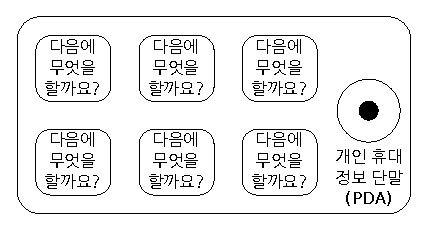
\includegraphics[height=1.00in]{figs2/pda2.eps}}
\afterfig

우선은 프로그래을 만드는 주된 동기가 사업을 위한다던가 사용자를 기쁘게 한다기 보다는 일상생활에서 맞닥드리는 자료와 정보를 잘 다뤄 좀더 생산적으로 우리의 삶을 만드는데 초점을 잡아보자. 프로그램을 만들기 시작할 때 여러분 모두는 프로그래머이면서 동시에 자신이 만든 프로그램의 사용자가 된다. 프로그래머로서 기술을 습득하고 프로그래밍 자체로 창의적으로 느껴진다면, 여러분은 다른 사람을 위해 프로그램을 개발하게 준비가 된 것이다.

\section{컴퓨터 하드웨어 아키텍처}
\index{hardware}
\index{hardware!architecture}

소프트웨어 개발을 위해 컴퓨터에 지시 명령어를 전달하기 위한 컴퓨터 언어를 배우기 전에, 컴퓨터가 어떻게 구성되어 있는지 이해할 필요가 있다. 컴퓨터 혹은 핸드폰을 분해해서 안쪽을 살펴보면, 다음의 주요 부품을 발견할 수 있다.

\beforefig
\centerline{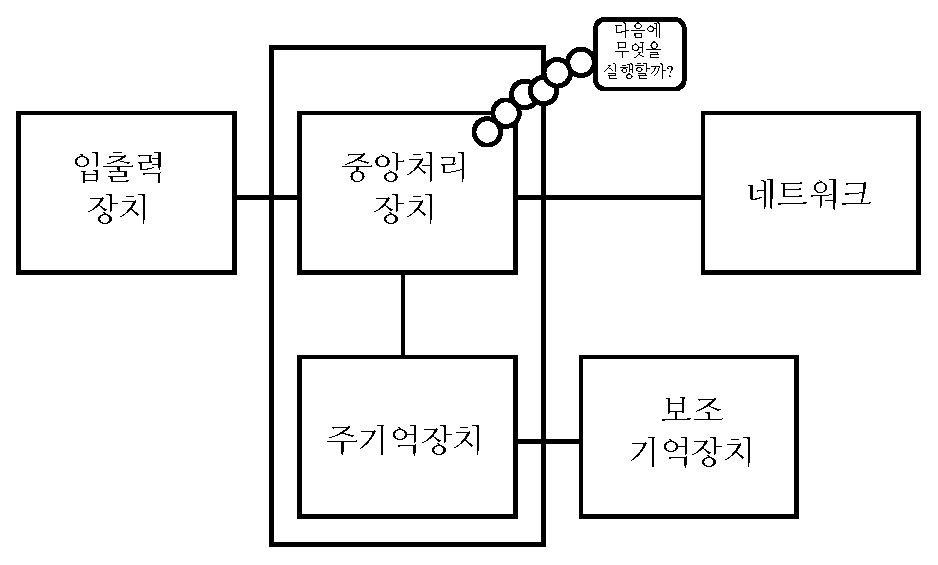
\includegraphics[height=2.50in]{figs2/arch.eps}}
\afterfig

주요 부품을 살펴보자.

\begin{itemize}

\item {\bf 중앙처리장치(Central Processing Unit, CPU): 다음은 무엇을 할까요? ("What is next?")} 명령어를 처리하는 주요 부분이다. 컴퓨터가 3.0 GHz라면 초당 명령어(다음은 무엇을 할까요? What is next?)를 삼백만번 처리할 수 있다고 계속 물을 수 있다. CPU의 처리속도를 따라서 컴퓨터와 빠르게 대화하는 것을 배울 것이다.

\item {\bf 주 기억장치(Main Memory):} 주기억장치는 중앙처리장치(CPU)가 급하게 명령어를 처리하기 위해 필요로 하는 정보를 저장하는 용도로 사용된다. 주 기억장치는 중앙처리장치만큼이나 빠르다. 그러나 주기억장치에 저장된 정보는 컴퓨터가 꺼지면 자동으로 지워진다.

\item[보조 기억장치] 보조 기억장치는 정보를 저장하기 위해 사용되지만, 주기억장치보다 속도가 느리다. 
전기가 나갔을 때도 정보를 기억하는 것이 장점이다. 휴대용 USB 기억장치나 이동 MP3 플레이어에 사용되는 USB의 플래쉬 메모리나 디스크 드라이브가 여기에 속한다.
 
\item {\bf 입출력장치(Input Output Devices):} 간단하게 화면, 키보드, 마우스, 마이크, 스피커, 터치패드가 포함된다. 컴퓨터와 사람이 상호작용하는 방식이다.

\item {\bf 네트워크(Network):} 요즘 거의 모든 컴퓨터는 네트워크로 정보를 주고 받는 네트쿼크 커넥션(Network Connection) 하드웨어를 가지고 있다. 네트워크는 정보를 저장하는 느린 저장소로 혹은 때때로 원하는 정보를 가져오지 못하는 것으로 보조 기억장치(Secondary memory)로 생각할 수 있다.

\end{itemize}
 

어떻게 이러한 주요 부품들이 작동하는지에 대한 자세한 사항은 컴퓨터를 만드는 사람에게 달려있지만, 프로그램을 만들때 컴퓨터 주요부품에 대해서 언급되어 컴퓨터 전문용어를 습득하고 이해하는 것은 도움이 된다.

프로그래머로서 여러분들은 사용자가 원하는 자료를 분석하고 문제를 풀 수 있는 컴퓨터 자원들을 사용하고 오케스트레이션하는 것이다.


\beforefig
\centerline{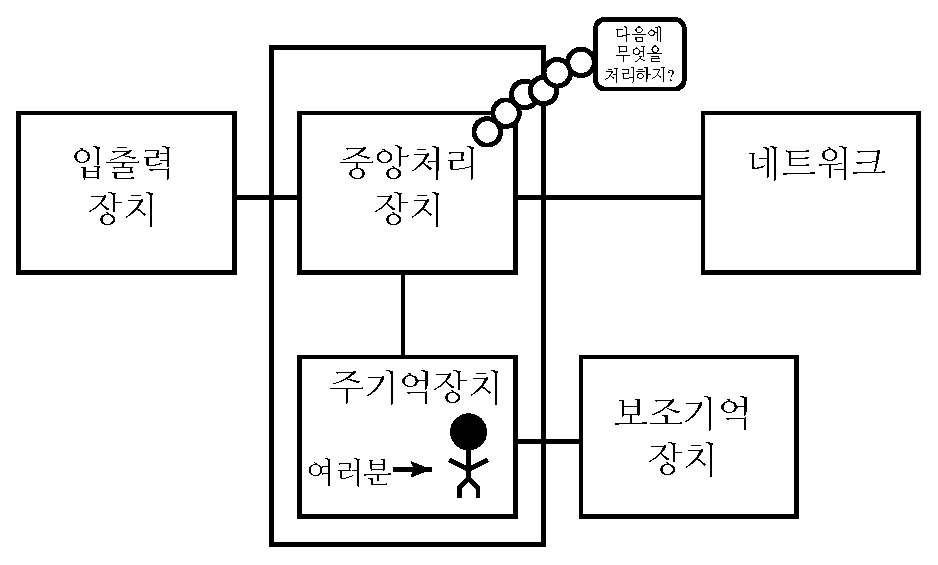
\includegraphics[height=2.50in]{figs2/arch2.eps}}
\afterfig

프로그래머로 중앙처리장치(CPU)와 대화하며 "다음은 무엇을 수행하세요"라고 지시할 것이다. 때때로 중앙처리장치(CPU)에게 주 기억장치, 보조 기억장치, 네트워크, 입출력 장치를 사용하라고 지시할 것이다.

프로그래머는 컴퓨터의 "다음은 무엇을 수행할까요"에 대한 답을 하는 사람이기도 하다. 하지만, 컴퓨터에 답하기 위해서 5mm 크기로 컴퓨터에 프로그래머를 집어넣고 초당 30억개의 명령어로 답을 하는 것은 매우 불편할 것이다. 그래서, 미리 컴퓨터에게 수행할 명령문을 써놔야한다. 이렇게 미리 작성된 명령문의 집합을 {\bf 프로그램(Program)}이라고 하며, 명령어 집합을 작성하고 명령어 집합이 올바르게 작성될 수 있도록 하는 행위를 {\bf 프로그래밍(Programming)}이라고 부른다.



\section{프로그래밍 이해하기}

책의 나머지 장을 통해서 책을 읽고 있는 당신을 프로그래밍의 장인으로 인도할 것입니다. 종국에는 책을 읽고 있는 여러분은 {\bf 프로그래머}가 될 것입니다. 아마도 전문적인 프로그러머는 아닐지라도 적어도 자료/정보 분석 문제를 보고 그 문제를 풀수 있는 기술을 가지게는 될 것입니다.

\index{problem solving}

이런 점에서 프로그래머가 되려면 두가지 기술이 필요로 합니다.

\begin{itemize}

\item 첫째, 파이썬같은 프로그래밍 언어 - 어휘와 문법을 알 필요가 있습니다. 단어를 새로운 언어에 맞추어 쓸 수 있어야 하며 새로운 언어를 잘 표현된 문장으로 구성하는지를 알아야 합니다.

\item 둘째, 스토리(Story)를 말 할 수 있어야 합니다. 스토리를 만들때, 독자에게 우리의 아이디어(idea)를 전달하기 위해서 단어와 문장을 조합합니다. 스토리를 만들 때 기술과 예술적인 면이 있으며, 기술과 예술적인 면은 여러번 쓰기 연습을 통하고 피트백을 받으므로써 향상됩니다. 프로그래밍에서, 우리가 만든 프로그램은 스토리이고, 풀려고 하는 문제는 "아이디어"에 해당합니다.

\end{itemize}

파이썬과 같은 프로그래밍 언어를 배우게 되면, 자바스크립트나 C++ 같은 두번째 언어를 배우는 것은 무척이나 쉽습니다. 새로운 프로그래밍 언어는 매우 다른 어휘와 문법을 가지지만, 문제푸는 기술을 배우기만 하면, 모든 프로그래밍 언어에서로 동일하게 접근할 수 있습니다.

파이썬의 어휘와 문단은 금방 배웁니다. 새로운 종류의 문제를 풀기위해 논리적인 프로그램을 짜는 것은 오래 걸립니다. 여러분은 작문을 배우듯이 프로그래밍을 배우게 될 것입니다. 프로그래밍을 읽고 설명하는 것으로 시작해서 간단한 프로그램을 작성하고, 점차적으로 복잡한 프로그램을 작성하게될 것입니다. 어느 순간에 명상에 잠기게 되고, 문제해결과 프로그램의 패턴을 보게되고, 좀더 자연스럽게 어떻게 문제를 받아들여 그 문제를 해결할 수 있는 프로그램을 작성하게 될 것입니다. 그리고, 그 순간에 도착하게 되면, 프로그래밍은 매우 즐겁고 창의적인 과정이 될 것입니다.

파이썬 프로그램의 어휘와 구조로 시작을 합니다. 간단한 예제가 언제 처음으로 프로그램을 읽기 시작했는지를 일깨워 주니 인내심을 가지세요.

\section{단어와 문장}
\index{programming language}
\index{language!programming}

사람의 언어와 달리, 파이썬의 어휘는 실질적으로 매우 적다. 어휘를 예약어(researved words)로 부른다. 이들 단어는 파이썬에 매우 특별한 의미를 가진다. 파이썬 프로그램에서 파이썬이 이들 단어를 보게되면, 이들 단어는 파이썬에게 단 하나의 유일한 의미를 지니게 된다. 후에 여러분들이 프로그램을 작성할 때 여러분들이 만든 자신만의 단어를 작성하게 되는데 이를 {\bf 변수(Variable)}라고 합니다. 여러분의 변수의 이름을 지을 때 폭넓은 자유를 가질 수 있지만, 변수의 이름으로 파이썬의 예약어를 사용할 수는 없습니다.

이런 점에서 강아지를 훈련시킬 때 "앉아", "기달려", 가져와 같은 특별한 어휘를 사용합니다. 강아지에게 이런 특별한 예약어를 사용하지 않을 때, 강아지는 주인이 특별한 어휘를 사용하지 않을 때 주인을 물끄러미 쳐다보기만 합니다. 예를 들어, "여러분이 더 많은 사람들이 건강을 전반적으로 향상하는 방향으로 가자 원한다"고 말하면, 강아지가 든는 것은 ''뭐라 뭐라 뭐라 {\bf walk} 뭐라'' 이렇게 들릴 것이다. 왜냐하면 "가자"가 강아지의 언어에는 예약어\footnote{\url{http://xkcd.com/231/}}이기 때문이다. 이러한 사실은 개와 사람사이에는 예약어가 없다는 것을 의미할지도 모른다.

사람이 파이썬에게 말을 하는 예약어는 다음과 같은 것이 있다.

\beforeverb
\begin{verbatim}
and       del       from      not       while    
as        elif      global    or        with     
assert    else      if        pass      yield    
break     except    import    print              
class     exec      in        raise              
continue  finally   is        return             
def       for       lambda    try
\end{verbatim}
\afterverb
%
강아지의 사례와는다르게 파이썬은 이미 완벽하게 훈련이 되어 있다. 여러분이 "try" 라고 말하면, 파이썬은 여러분이 매번 "try" 라고 말할 때마다 실패 없이 시도를 할 것이다.

이러한 예약어를 배울 것이고 어떻게 잘 사용되는지도 함께 배울것이지만, 지금은 파이썬에 말하는 것에 집중할 것이다. 파이썬에게 말하는 것 중 좋은 것은 다음과 같은 메세지를 던지는 것으로도 파이썬에 말을 할 수 있다는 것이다.

\beforeverb
\begin{verbatim}
print 'Hello world!'
\end{verbatim}
\afterverb

이 간단한 문장이 파이썬의 구문(Syntax)론적으로 완벽하다. 위 문장은 예약어 'print'로 시작해서 출력하고자 하는 문자열을 작은 따옴표로 감싸안아 올바르게 파이썬에게 전달했다.

\section{파이썬과 대화하기}

파이썬으로 우리가 알고 있는 단어를 가지고 간단한 문장을 만들었고, 새로운 언어 기술을 시험하기 위해서 파이썬과 대화를 어떻게 하는지 알 필요가 있다.

파이썬과 대화를 시작하기 전에, 파이썬 소프트웨어를 컴퓨터에 설치하고 컴퓨터에서 파이썬을 어떻게 실행하는지를 배워야 한다. 이번장에서 다루기에는 너무 구체적이고 자세한 사항이기 때문에 \url{www.pythonlearn.com}을 참조하는 것을 권고한다. 자세한 설치 방법과 화면을 캡쳐하여 윈도우와 매킨토쉬 시스템 및 실행하는 방법을 설명하였다. 설치가 마무리되고 터미널이나 명령어 실행창에서 {\bf python}을 치게되면 파이썬 인터프리터가 인터랙티브 모드로 실행을 시작하고 다음과 같은 것이 화면에 뿌려진다.

\index{interactive mode}

\beforeverb
\begin{verbatim}
Python 2.6.1 (r261:67515, Jun 24 2010, 21:47:49) 
[GCC 4.2.1 (Apple Inc. build 5646)] on darwin
Type "help", "copyright", "credits" or "license" for more information.
>>> 
\end{verbatim}
\afterverb
%
{\tt >>>} 프롬프트는 파이썬 인터프리터가 여러분에게 요청하는 방식이다. "다음에 파이썬이 무엇을 실행하기를 원합니까?" 파이썬은 여러분과 대화를 나눌 준비가 되었다. 이제 남은 것은 파이썬 언어로 어떻게 말하는 지를 여러분이 아는 것이고 여러분은 대화를 할 수 있다.

예를들어 여러분이 가장 간단한 파이썬 언어의 단어나 문장 조차도 알수가 없다고 가정해 봅시다. 우주 비행사가 저 멀리 떨어진 행성에 착륙할 때 사용하는 간단한 말을 사용하여 행성의 거주민에게 대화를 시도한다고 생각해 봅시다.

\beforeverb
\begin{verbatim}
>>> I come in peace, please take me to your leader
  File "<stdin>", line 1
    I come in peace, please take me to your leader
         ^
SyntaxError: invalid syntax
>>> 
\end{verbatim}
\afterverb
%
잘 되는것 같지 않습니다. 뭔가 빨리 다른 생각을 하지 않는다면, 행성의 거주민은 창으로 찔르고, 기름에 잘 발라 불위에서 바베큐를 만들어 저녁으로 먹을 듯 합니다.

운 좋게도 기나긴 우주 여행중 이책의 복사본을 가지고 와서 다음과 같이 빠르게 친다고 생각해봅시다.

\beforeverb
\begin{verbatim}
>>> print 'Hello world!'
Hello world!
\end{verbatim}
\afterverb
%

훨씬 좋아보기고, 좀더 커뮤니케이션을 이어갈 수 있을 것으로 보입니다.

\beforeverb
\begin{verbatim}
>>> print 'You must be the legendary god that comes from the sky'
You must be the legendary god that comes from the sky
>>> print 'We have been waiting for you for a long time'
We have been waiting for you for a long time
>>> print 'Our legend says you will be very tasty with mustard'
Our legend says you will be very tasty with mustard
>>> print 'We will have a feast tonight unless you say
  File "<stdin>", line 1
    print 'We will have a feast tonight unless you say
                                                     ^
SyntaxError: EOL while scanning string literal
>>> 
\end{verbatim}
\afterverb
%

이번 대화는 잠시동안 잘 진행되다가 여러분이 파이썬 언어로 말하다가 정말 사소한 실수를 저질러 파이썬이 오류를 뱉어낸다.

이번에 파이썬이 놀랍도록 복잡하고 강력하고 파이썬과 의사소통을 할때 사용하는 신택스(syntax)가 매우 까다롭다는 것은 알 수 있었다. 파이썬은 다른말로 똑똑(Intelligent)하지는 않다. 지금까지 여러분은 자신과 대화를 저절한 신택스(syntax)를 가지고 대화를 했습니다.

여러분이 다른사람이 작성한 프로그램을 사용한다는 것은 여러분과 파이썬을 사용하는 다른 프로그래머가 파이썬을 중간 매개체로 대화를 하는 것으로 볼 수 있습니다. 파이썬은 프로그램을 만든 저작자가 어떻게 대화가 진행되어져야 하는지를 표현하는 방식입니다. 다음 몇 장에 걸쳐서 여러분은 파이썬을 이용하여 여러분의 프로그램을 이용하는 다른 많은 프로그래머 중의 한명이 될 것입니다.

파이썬 인터프리터와 대화하는 첫 장을 끝내기 전에, 파이썬 행성의 거주자에게 "안녕히 계세요"를 말하는 적절한 방법을 알아야 한다.

\beforeverb
\begin{verbatim}
>>> good-bye
Traceback (most recent call last):
  File "<stdin>", line 1, in <module>
NameError: name 'good' is not defined

>>> if you don't mind, I need to leave
  File "<stdin>", line 1
    if you don't mind, I need to leave
             ^
SyntaxError: invalid syntax

>>> quit()
\end{verbatim}
\afterverb
%
위 처음 두개의 시도는 다른 오류 메세지를 출력한다. 두번째 오류는 다른데 이유는 {\bf if}가 예약어이기 때문에 파이썬은 이 예약어를 보고 뭔가 다른 것을 말한다고 생각하지만, 잠시 후 문장의 신택스가 잘못됐다고 판정하고 오류를 뱉어낸다.

파이썬에게 "안녕히 계세요"를 말하는 올바른 방식은 인터렉티브 {\tt >>>} 프롬프트에서 {\bf quit()}를 입력하는 것이다.



\section{전문용어: 인터프리터와 컴파일러}
파이썬은 사람이 읽고 쓸수 있고 컴퓨터도 읽고 쓸 수 있도록 고안된 {\bf 하이레벨(High-level)} 언어이다. 다른 하이레벨 언어는 자바, C++, PHP, 루비, 베이직, 펄, 자바스크립트 등 다수가 있다. 중앙처리장치(CPU)내에서 실제 하드웨어 수준에서 이런 하이레벨 언어를 이해하지 못한다.

중앙처리장치는 우리가 {\bf 기계어(machine-language)}로 부르는 언어만 이해한다. 기계어는 매우 간단하고 솔직히 작성하기에는 매우 지루하다. 왜냐하면 모두 0과 1로만 표현되기 때문이다.

\beforeverb
\begin{verbatim}
01010001110100100101010000001111
11100110000011101010010101101101
...
\end{verbatim}
\afterverb
%
0과 1로만 되어 있기 때문에 기계어가 간단해 보이지만, 시택스는 복잡하고 파이썬보다 훨씬 어렵다. 그래서 매우 소수의 프로그래머만이 기계어를 쓸수 있다. 대신에 파이썬과 자바스크립트 같은 하이레벨 언어로 프로그래머가 작성할 수 있도록 다양한 번역기(translator)를 만들었다. 이들 번역기는 프로그램을 중앙처리장치에 의해서 실제 실행이 가능한 기계어로 변환하여 준다.

기계어는 컴퓨터하드웨어에 묶여있기 때문에 기계어는 다른 형식의 하드웨어에 {\bf 이식(portable)}이 되지 않는다. 하이레벨 언어로 작성된 프로그램은 새로운 하드웨어위에 다른 인터프리터를 이용하여 옮겨 실행이 가능하고 다른 하드웨어에 사용할 수 있도록 프로그램을 다시 컴파일하여 사용할 수 있다.

프로그래밍 언어의 번역기는 두가지 범주가 있다. 
(1) 인터프리터 (2) 컴파일러

{\bf 인터프리터}는 프로그래머에 의해서 쓰여진 소스코드를 읽고, 소스코드를 파싱하고, 즉석에서 명령어를 해석한다. 파이썬은 인터프리터다. 파이썬을 인터렉트브 모드로 실행할때, 파이썬 명령문을 쓰면, 파이썬이 즉성에서 처리하고, 다른 파이썬 명령어를 여러분으로부터 기다린다.

파이썬 명령어는 파이썬이 나중에 사용될 값을 기억하기를 바란다. 적당한 이름을 잡아서 그 값을 기억시키고, 나중에 그 이름을 호출하여 값을 사용할 수 있다. 이러한 목적으로 값을 저장하는 것을 {\bf 변수(variable)}라고 한다.

\beforeverb
\begin{verbatim}
>>> x = 6
>>> print x
6
>>> y = x * 7
>>> print y
42
>>> 
\end{verbatim}
\afterverb
%
이 예제에서 파이썬이 x라는 라벨을 사용하여 6이라는 값을 저장하기를 바라고 나중에 사용코저 한다. {\bf print} 예약어를 사용하여 파이썬이 잘 기억하고 있는지를 검증한다. 그리고 {\bf x}를 반환하여 7을 곱하고 새로운 변수 {\bf y}에 값을 집어 넣는다. 그리고 {\bf y}에 현재 무엇이 저장되어 있는지 출력하라고 파이썬에게 요청한다.

파이썬에 한줄 한줄 명령어를 쳐 넣고 있지만, 파이썬은 앞쪽에 명령문에서 생성된 자료가 나중의 실행 명령문에서 사용될 수 있도록 정렬된 명령문으로 처리한다. 방금전 논리적이고 의미있는 순서로 4줄의 명령문을 가진 한 단락을 작성한 것이다.

위에서 본것처럼 파이썬과 대화를 주고받을 수 있는 것이 {\bf 인터프리터}의 본질이다. {\bf 컴파일러}는 완전한 프로그램을 하나의 파일에 담겨지고, 하이레벨 소스코드가 기계어로 번역되고, 컴파일러가 나중에 실행되도록 기계어를 파일에 담아놓는다.

윈도우를 사용한다면, 실행가능한 기계어 프로그램의 확장자가 ".exe"(executable), 혹은 ".dll"(dynamically loadable library)임을 확인할 수 있다. 리눅스와 매키토쉬에서는 실행화일을 의미하는 확장자는 없다.

텍스트 편집기에서 실행파일을 열게되면 다음과 같은 읽을 수 없는 좀 괴상한 출력을 화면상에서 확인할 수 있다.

\beforeverb
\begin{verbatim}
^?ELF^A^A^A^@^@^@^@^@^@^@^@^@^B^@^C^@^A^@^@^@\xa0\x82
^D^H4^@^@^@\x90^]^@^@^@^@^@^@4^@ ^@^G^@(^@$^@!^@^F^@
^@^@4^@^@^@4\x80^D^H4\x80^D^H\xe0^@^@^@\xe0^@^@^@^E
^@^@^@^D^@^@^@^C^@^@^@^T^A^@^@^T\x81^D^H^T\x81^D^H^S
^@^@^@^S^@^@^@^D^@^@^@^A^@^@^@^A\^D^HQVhT\x83^D^H\xe8
....
\end{verbatim}
\afterverb
%
It is not easy to read or write machine language so it is nice that we have
{\bf interpreters} and {\bf compilers} that allow us to write in a high-level
language like Python or C.

Now at this point in our discussion of compilers and interpreters, you should 
be wondering a bit about the Python interpreter itself.  What language is 
it written in?  Is it written in a compiled language?  When we type
``python'', what exactly is happening?

The Python interpreter is written in a high level language called ``C''.  
You can look at the actual source code for the Python interpreter by
going to \url{www.python.org} and working your way to their source code.
So Python is a program itself and it is compiled into machine code and
when you installed Python on your computer (or the vendor installed it),
you copied a machine-code copy of the translated Python program onto your
system.   In Windows the executable machine code for Python itself is likely
in a file with a name like:

\beforeverb
\begin{verbatim}
C:\Python27\python.exe
\end{verbatim}
\afterverb
%
That is more than you really need to know to be a Python programmer, but
sometimes it pays to answer those little nagging questions right at 
the beginning.

\section{프로그램 작성하기}

파이썬 인터프리터에 명령어를 치는 것은 파이썬의 주요기능을 알아볼 수 있는 좋은 방법이지만 좀더 복잡한 문제를 해결하기 위해서는 권해드리지는 않습니다.

프로그램을 작성할 때 {\bf 스크립트(script)}로 불리는 파일에 명령어 집합을 작성하기 위해서 텍스트 편집기를 주로 사용합니다. 파이썬 스크립트는 {\tt .py}라는 확장자를 가집니다.

\index{script}

스크립트를 실행하기 위해서 파이썬 인터프리터에게 파일의 이름을 말해줍니다. 유니스나 윈도우 명령창에서 {\tt python hello.py}를 치게 되면 다음과 같은 결과를 얻게 됩니다.

\beforeverb
\begin{verbatim}
csev$ cat hello.py
print 'Hello world!'
csev$ python hello.py
Hello world!
csev$
\end{verbatim}
\afterverb
%
''csev\$''은 운영시스템의 명령어 프롬프트이고, ''cat hello.py''는 문자열을 출력하라는 한줄의 파이썬 프로그램을 표시하라는 명령어입니다.

인터랙트브 모드로 파이썬 코드를 보여달라는 방식 대신에 파이썬 인터프리터를 호출하고 ''hello.py'' 파일에서 소스코드를 읽으라고 말하는 것입니다.

이 새로운 방식은 파이썬 프로그램을 끝내기 위해 {\bf quit()}를 사용할 필요가 없는 것이 좋은 점입니다. 파이썬이 파일에서 소스코드를 읽을 때, 파일 끝까지 읽게되면 파이썬은 자동으로 끝낼 줄을 알고 있습니다.

\section{프로그램이란 무엇인가?}

{\bf 프로그램(Program)}의 가장 기본적인 정의는 어떠한 일을 할 수 있도록 조작된 일련의 파이썬 명령문의 집합이다. 가장 간단한 {\bf hello.py} 스크립트도 프로그램이다. 한줄의 프로그램으로 특별히 유익하고 쓸모가 있는 것은 아니지만 엄격한 의미에서 파이썬 프로그램이 맞다.

프로그램을 이해하는 가장 쉬운 방법은 프로그램이 어떠한 문제를 풀려고 만들어졌는지 문제를 먼저 생각하는 것이다. 그리고 그 문제를 풀려고 작성된 프로그램을 살펴보는 것이다.

예를 들어 여러분이 페이스북의 일련의 게시된 글에 가장 자주 사용된 단어에 관심을 가지고 소셜 컴퓨팅 연구를 한다고 생각해 봅시다. 페이스북에 게시된 글들을 출력하고 가장 흔한 단어를 찾으로 열심히 들여다 볼 것이지만 매우 오래걸리고 실수하기 쉽습니다. 하지만 파이썬 프로그램을 이용하면, 빨리 정확하게 작업을 할 수 있는 파이썬 프로그램을 작성해서 주말에 뭔가 재미있는 일로 보낼 수 있습니다.

예를 들어 다음의 자동차(car)와 광대(clown)를 보고, 가장 많이 나오는 단어는 무엇이며 몇번 나왔는지 세어보세요.

\beforeverb
\begin{verbatim}
the clown ran after the car and the car ran into the tent 
and the tent fell down on the clown and the car 
\end{verbatim}
\afterverb
%

그리고, 몇백만줄의 텍스트를 보고서 동일한 일을 한다고 상상해 보세요. 솔직히 수작업으로 단어를 세는 것보다 파이썬을 배워 프로그램을 배우는 것이 훨씬 빠를 것입니다.

더 좋은 소식은 이미 텍스트 파일에서 가장 자주 나오는 단어를 찾아내는 간단한 프로그램을 제시했고, 작성했고, 시험까지 했다. 이걸 가지고 여러분들은 바로 사용을 할 수 있기 때문에 수고를 덜 수 있다.

\beforeverb
\begin{verbatim}
name = raw_input('Enter file:')
handle = open(name, 'r')
text = handle.read()
words = text.split()
counts = dict()

for word in words:
   counts[word] = counts.get(word,0) + 1

bigcount = None
bigword = None
for word,count in counts.items():
    if bigcount is None or count > bigcount:
        bigword = word
        bigcount = count

print bigword, bigcount
\end{verbatim}
\afterverb
%
이 프로그램을 사용하려고 파이썬을 알 필요도 없다. 10장에 걸쳐서 멋진 파이썬 프로그램을 만드는 방법을 배우게 될 것입니다. 지금 여러분은 사용자로 단순히 프로그램을 사용하지만 이 프로그램이 얼마나 많은 수작업을 줄일 수 있는지 보여주고 있다. 코드를 작성하고 {\bf words.py}로 저장하여 실행을 하거나, \url{http://www.pythonlearn.com/code/}에서 소스코드를 다운로드 받아 실행하면 된다.

\index{program}
파이썬과 파이썬 언어가 중간의 중개자로서 여러분(사용자)과 저자(프로그래머)사이에서 중개자의 역할을 훌륭히 하고 있는 것을 보여주고 있습니다. 파이썬이 설치된 컴퓨터에서 누구나 사용할 수 있는 공통의 언어로 유용한 명령 순서(즉, 프로그램)를 주고받는지 보여준다. 그래서 {\em 파이썬과} 직접의사소통하지 않고 {\em 파이썬을 통해서} 서로 의사소통할 수 있다.

\section{프로그램 구성요소}

다음의 몇장에 걸쳐서 파이썬 어휘, 문장구조, 문단구조에 대해서 배울 것이다. 파이썬의 강력한 점에 대해서 배울 것이고, 유용한 프로그램을 작성하기 위해서 파이썬의 역량을 조합하는 법을 배울 것이다.

프로그램을 작성하기 위해서 사용하는 로우레벨(low-level) 패턴이 몇가지 있다. 파이썬을 위해서 만들어졌다기 보다는 기계어부터 하이레벨 언어에 이르기까지 모든 언어에 공통된 사항이다.

\begin{description}

\item[입력:] 컴퓨터 바깥세계에서 데이터를 가져온다. 파일로부터 데이터를 읽을 수도 있고, 마이크나 GPS 같은 센서에서 데이터를 입력받을 수도 있다. 위 프로그램에서 사용자의 키보드로 데이터를 입력받아 입력값으로 사용된 사례이다.

\item[출력:] 화면에 프로그램의 결과값을 보여주거나 파일에 저장한다. 혹은 음악을 연주하거나 텍스트를 읽도록 스피커 같은 장치에 데이터를 보낸다.

\item[순차 실행:] 스크립트에 작성된 순서에 맞추어 한줄 한줄 실행된다.

\item[조건 실행:] 조건을 확인하고 명령문을 실행하거나 건너뛴다.

\item[반복 실행:] 반복적으로 명령문을 실행한다. 대체로 반복 실행시 변화를 수반한다.

\item[재사용:] 명령어를 한번 작성하고 이름을 주어 저장하고 프로그램의 필요에 따라 이름을 불러 몇차례 다시 사용한다.

\end{description}

너무나 간단하게 들리지만, 전혀 간단하지는 않다. 걸음거리를 간단히 ''한 다리를 다를 다리 앞에 놓으세요'' 라고 말하는 것 같다. 프로그램을 짜는 ''예술''은 이러한 기본 요소를 조합하고 엮어 사용자에게 유용한 무언가를 만드는 것이다.

단어를 세는 프로그램은 위 프로그램의 기본요소를 하나만 빼고 모두 사용하여 작성되었다.


\section{프로그램이 잘못되면?}

파이썬과 처음에 대화를 할때, 파이썬 코드를 명확하게 작성하여 의사소통을 해야한다. 작은 차이 혹은 실수는 파이썬이 여러분이 작성한 프로그램을 보다가 포기하게 만듭니다.

초보 파이썬 프로그래머는 파이썬이 오류에 대해서는 인정사정볼 것 없다고 생각합니다. 파이썬이 모든 사람을 좋아하는 것 같지만, 파이썬은 사적으로 사람들을 알고 있고, 뒤끝이 있습니다. 이러한 사실로 인해서 파이썬은 완벽하게 작성된 프로그램만을 가지게 되고 ''잘못 작성되었어요''라고 뱉어내고 여러분에게 고통을 줍니다.

\beforeverb
\begin{verbatim}
>>> primt 'Hello world!'
  File "<stdin>", line 1
    primt 'Hello world!'
                       ^
SyntaxError: invalid syntax
>>> primt 'Hello world'
  File "<stdin>", line 1
    primt 'Hello world'
                      ^
SyntaxError: invalid syntax
>>> I hate you Python!
  File "<stdin>", line 1
    I hate you Python!
         ^
SyntaxError: invalid syntax
>>> if you come out of there, I would teach you a lesson
  File "<stdin>", line 1
    if you come out of there, I would teach you a lesson
              ^
SyntaxError: invalid syntax
>>> 
\end{verbatim}
\afterverb
%

파이썬과 다퉈봐야 얻을 것은 없어요. 파이썬은 도구고 감정이 없습니다. 여러분이 필요로 할 때마다 여러분에게 봉사하고 기쁨을 주기 위해서 존재할 뿐입니다. 오류 메세지가 심하게 들릴지는 모르지만 단지 파이썬이 도와달라고 하는 요청일 뿐입니다. 여러분이 입력한 것을 쭉 읽어보고 여러분이 입력한 것을 이해할 수 없다고만 말할 뿐입니다.

파이썬은 어떤면에서 강아지와 닮았습니다. 맹목적으로 여러분을 사랑하고, 강아지가 이해하는 몇몇 단어만 이해하며, 웃는 표정({\tt >>>} 명령 프롬프트)으로 여러분이 무언가를 말하기만을 기다립니다. 파이썬이 ''SyntaxError: invalid syntax''을 뱉어낼 때, 꼬리를 흔들면서 ''뭔가 말씀하시는 것 같은데요... 주인님 말씀을 이해하지 못하겠어요, 다시 말씀해 주세요 ({\tt >>>})'' 말하는 것과 같다.

여러분이 작성하는 프로그램이 점점 유용해지고 복잡해짐에 따라 3가지 유형의 오류를 마주치게 된다.

\begin{description}

\item[구문 오류(Syntax Error):]첫번째 마주치는 오류로 고치기 가장 쉽습니다. 구문 오류는 파이썬의 문법에 맞지 않는다는 것을 의미합니다. 파이썬은 구문오류가 발생한 줄을 찾아 정확한 위치를 알려줍니다. 하지만, 파이썬이 제시하는 오류가 그 이전 프로그램 부문에서 발생했을 수도 있기 때문에 파이썬이 알려주는 곳 뿐만 아니라 그 앞쪽도 살펴볼 필요가 있다. 따라서 파이썬이 제시하는 구문 오류의 경우 오류가 난 곳은 오류를 고치기 위한 시작점으로 의미가 있다.

\item[논리 오류(Logic Error):] 논리 오류는 프로그램의 구문은 완벽하지만 명령문의 실행에 혹은 다른 명령어부분과 관련된 부문에서 실수가 있는 것이다. 논리 오류의 예를 들어보자. ''물병에서 한모금 마시고, 가방에 넣고, 도서관으로 걸어가서, 물병을 닫는다''

\item[시맨틱 오류(Semantic Error):] 시맨틱 오류는 구문론적으로 완벽하고 올바른 순서로 프로그램의 명령문이 작성되었지만 프로그램에 오류가 숨어있다. 프로그램은 완벽하게 작동하지만 여러분이 의도한 바를 수행하지는 못합니다. 간단한 예로 여러분이 식당으로 가는 방향을 알려주고 있습니다. '' ... 주유소 사거리에 도착했을 때, 왼쪽으로 돌아 1.6km 쭉 가면 왼쪽편에 빨간색 빌딩에 식당이 있습니다.'' 친구가 매우 늦어 전화로 지금 농장에 있고 헛간으로 걸어가고 있는데 식당을 발견할 수 없다고 전화를 합니다. 그러면 여러분은 ''주유소 왼쪽 혹은 오른쪽을 돈거야'' 말하면, 그 친구는 ''말한대로 완벽하게 따라서 했고, 말한대로 적기까지 했는데, 왼쪽으로 돌아 1.6km에 주요소가 있다고 했어'', 그러면 여러분은 ''미안해, 내가 가지고 있는 건 구문론적으로는 완벽한데, 사소한 시맨틱 오류가 있네!'' 라고 말할 것이다.

\end{description}

위 세 종류의 오류에 대해서 파이썬은 여러분이 요청한 것을 충실히 수행하기 위해서 최선을 다합니다.

\section{학습으로의 여정}

여러분이 책을 읽으면서 개념들이 처음에 잘 와 닿지 않는다고 기죽을 필요는 없어요. 여럽누이 말하는 것을 배울 때, 처음 몇년동안 웅얼거리는 것은 문제가 아닙니다. 간단한 어휘에서 간단한 문장으로 옮겨가고, 문장에서 문단으로 옮겨가는데 6개월이 걸려도 괜찮습니다. 흥미로운 완벽한 짧은 스토리를 자신의 언어로 작성하는데 몇 년이 걸립니다.

여러분이 파이썬을 빨리 배울수 있도록 다음의 몇장에 걸쳐서 정보를 제공해 드릴 것입니다. 새로운 언어를 습득하는 것과 같아서 자연스럽게 느껴지기까지 흡수하고 이해하기까지 시간이 걸립니다. 큰 그림(Big Picture)을 이루는 작은 조각을 정의하면서 여러분을 큰 그림을 볼 수 있도록 여러 주제를 찾고, 또 찾으면서 혼란이 생길 수 있다. 이책이 순차 선형적으로 쓰여져서 본 과정을 선형적으로 배워갈 수도 있지만, 비선형적으로 본 교재를 활용하는 것도 괜찮다. 가볍게 앞쪽과 뒷쪽을 넘나들며 책을 읽을 수도 있다. 구체적이고 세세한 점을 완벽하게 이해하지 않고 고급 과정을 가볍게 읽으면서 프로그래밍의 ''왜(Why)''에 대해서 더 잘 이해할 수도 있다. 앞에서 배운것을 다시 리뷰하고 앞의 연습문제를 다시 하면서 처음에 난공불락이라 여겼던 어려운 주제도 더잘 배우고 이해할 수 있다는 것을 알게될 것이다.

대체적으로 처음 프로그래밍 언어를 배울 때 망치로 돌을 내리치고, 끌로 깎아내고 하면서 아름다운 조각품을 만들면서 겪게되는 몇 번의 '' 유레카, 아 하~~'' 순간이 있다.

만약 어떤 것이 특별히 힘들다면, 밤새도록 앉아서 지켜보고 노력하는 것은 별로 의미가 없다. 잠시 쉬고, 낮잠을 자고, 간식을 먹고 다른사람이나 강아지에게 문제를 설명하고 자문을 구한 후에 깨끗한 정신과 눈으로 돌아와서 다시 시도해보라. 단언컨데 이책의 프로그래밍 개념을 배우자마자 정말 쉽고 멋지다는 것을 돌이켜 보면 알게될 것이다. 프로그래밍 언어는 정말 배울 가치가 있다.

\section{용어사전}

\begin{description}

\item[버그(bug):]  프로그램 오류
\index{bug}

\item[중앙처리장치(central processing unit, CPU):] 컴퓨터의 심장, 여러분이 작성한 프로그램을 실행하는 장치, "CPU" 혹은 프로세서라고 불립니다.
\index{central processing unit}
\index{CPU}

\item[컴파일러(compile):]  하이레벨 언어로 작성된 프로그램을 로우레벨 언어로 즉시 혹은 나중에 사용하도록 번역하는 번역기
\index{compile}

\item[하이레벨 언어(high-level language):]  사람이 읽고 쓰기 쉽게 설계된 파이썬과 같은 프로그래밍 언어
\index{high-level language}

\item[인터랙티브 모드(interactive mode):] 프롬프트에서 명령어나 표현식을 입력함으로써 파이썬 인터프리터를 사용하는 방식
\index{interactive mode}

\item[인터프리트(interpret):] 하이레벨 언어의 프로그램을 한번에 한줄씩 번형해서 실행하는 것
\index{interpret}

\item[로우레벨 언어(low-level language):] 컴퓨터가 실행하기 쉽게 설계된 프로그래밍 언어, ''기계어 코드'', ''어셈블리 언어''로 불린다.
\index{low-level language}

\item[기계어 코드(machine code):] 중앙처리장치에 의해서 바로 실행될수 있는 가장 낮은 수준의 언어로된 소프트웨어
\index{machine code}

\item[주메모리(main memory):] 프로그램과 데이터를 저장한다. 전기가 나가게 되면 주메모리에 저장된 정보는 사라진다.
\index{main memory}

\item[파싱(parse):]  프로그램을 검사하고 구문론적 구조를 분석하는 것
\index{parse}

\item[이식(portability):] 하나 이상의 컴퓨터에서 실행될 수 있는 프로그램의 특성
\index{portability}

\item[출력문(print statement):] 파이썬 인터프리터가 화면에 값을 출력할 수 있게 만드는 명령문
\index{print statement}
\index{statement!print}

\item[문제해결(problem solving:)] 문제를 만들고, 답을 찾고, 답을 표현하는 과정
\index{problem solving}

\item[프로그램(program:)] 컴퓨테이션(Computation)을 명세하는 명령어의 집합
\index{program}

\item[프롬프트(prompt):] 프로그램이 메세지를 출력하고 사용자가 프로그램에 입력하도록 기다릴 때.
\index{prompt}

\item[보조 기억장치] 전기가 나갔을 때도 정보를 기억하고 프로그램을 저장하는 저장소. 일반적으로 주메모리보다 속도가 느리다. USB의 플래쉬 메모리나 디스크 드라이브가 여기에 속한다.
\index{secondary memory}

\item[시맨틱(semantics):]  프로그램의 의미
\index{semantics}

\item[시맨틱 오류(semantic error):]  프로그래머가 의도한 것과 다른 행동을 하는 프로그램의 오류
\index{semantic error}

\item[소스코드(source code):]  하이레벨 언어로 기술된 프로그램
\index{source code}

\end{description}

\section{연습문}


\begin{ex}
컴퓨터 보조기억장치의 기능은 무엇입니까?

a) 모든 연산과 프로그램의 로직을 수행한다.\\
b) 인터넷의 웹페이지를 불러온다.\\
c) 파워가 없을 때도 장시간 정보를 저장한다.\\
d) 사용자로부터 입력정보를 받는다.
\end{ex}

\begin{ex}
프로그램은 무엇입니까?
\end{ex}

\begin{ex}
컴파일러와 인터프리터의 차이점을 설명하세요.
\end{ex}

\begin{ex}
기계어 코드는 다음중 어는 것입니까?

a) 파이썬 인터프리터\\
b) 키보드\\
c) 파이썬 소스코드 파일\\
d) 워드 프로세싱 문서
\end{ex}

\begin{ex}
 다음 코드에서 잘못된 점을 설명하세요.

\beforeverb
\begin{verbatim}
>>> primt 'Hello world!'
  File "<stdin>", line 1
    primt 'Hello world!'
                       ^
SyntaxError: invalid syntax
>>> 
\end{verbatim}
\afterverb

\end{ex}

\begin{ex}
다음의 파이썬 프로그램이 실행된 후에 변수 "X"는 어디에 저장됩니까?

\beforeverb
\begin{verbatim}
x = 123
\end{verbatim}
\afterverb
%
a) 중앙처리장치\\
b) 주메모리\\
c) 보조메모리\\
d) 입력장치\\
e) 출력장치
\end{ex}

\begin{ex}
다음 프로그램에서 출력되는 것은 무엇입니까?

\beforeverb
\begin{verbatim}
x = 43
x = x + 1
print x
\end{verbatim}
\afterverb
%
a) 43\\
b) 44\\
c) x + 1\\
d) 오류, 왜냐하면 x = x + 1 은 수학적으로 불가능하다.
\end{ex}

\begin{ex}
사람의 어느 능력부위에 해당하는지 예로하여 다음을 설명하세요.
(1) 중앙처리장치, (2) 주메모리, (3) 보조메모리, 
(4) 입력장치
(5) 출력장치
중앙처리장치에 상응하는 사람의 몸 부위는 어디입니까? 
\end{ex}

\begin{ex}
구문오류("Syntax Error")는 어떻게 고칩니까?
\end{ex}

